% !TEX ROOT = ./distributed_mrf.tex
\section{Background}\label{sec:background}

\begin{figure}[t]
  \centering
  \begin{small}
    \begin{small}
  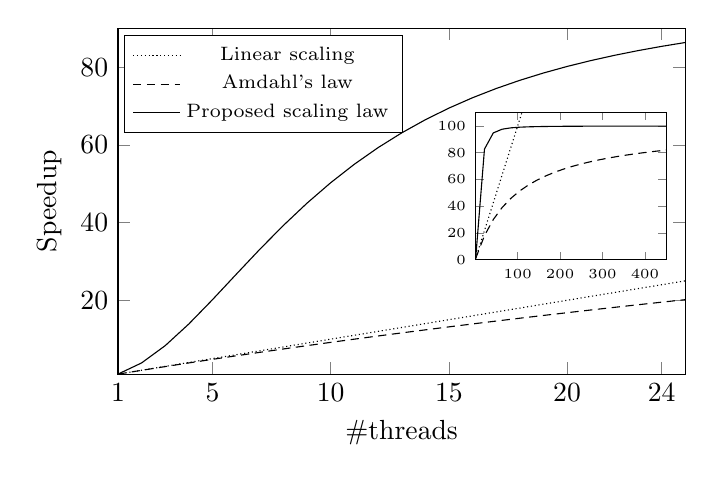
\begin{tikzpicture}[remember picture]
    \begin{axis}[
      width=250pt,
      height=170pt,
      xlabel={\#threads},
      ylabel={Speedup},
      xlabel near ticks,
      ylabel near ticks,
      xmin=1,
      xmax=25,
      ymin=1,
      ymax=90,
      xtick={1,5,10,15,20,24},
      legend style = {
        anchor = north west,
        at = {(rel axis cs:0.01,0.98)},
        font=\scriptsize,
        % draw = none,
      },
      no markers
      ]
      % use TeX as calculator:
      \addplot[domain=1:25,black,densely dotted]{x};
      \addlegendentry{Linear scaling}

      \addplot[domain=1:25,black,densely dashed]{1/(0.01 + (1-0.01)/x)};
      \addlegendentry{Amdahl's law}

      \addplot[domain=1:25,black,solid]{1/(0.01 + (1-0.01)/x^2)};
      \addlegendentry{Proposed scaling law}

      \coordinate (insetPosition) at (rel axis cs:.97,0.25);
      % \addplot[domain=0:15,black,loosely dashed]{1/(0.4 + (1-0.4)/x)};
      % \addlegendentry{Amdahl's law ($\delta=0.4$)}

      % \addplot[domain=0:15,black,loosely dotted]{1/(0.4 + (1-0.4)/x^2)};
      % \addlegendentry{Proposed scaling law for MTF ($\delta=0.4$)}
    \end{axis}
    \begin{axis}[
      at={(insetPosition)},
      anchor={outer south east},
      width=105pt,
      height=85pt,
      tiny,
      % xlabel={\#cores},
      % ylabel={Speedup},
      xmin=1,
      xmax=450,
      ymin=0,
      ymax=110,
      % ytick={1,2,3,4,5},
      no markers]
      \addplot[domain=1:500,black,densely dotted]{x};
      \addplot[domain=1:500,black,densely dashed]{1/(0.01 + (1-0.01)/x)};
      \addplot[domain=1:500,black,solid]{1/(0.01 + (1-0.01)/x^2)};
    \end{axis}
  \end{tikzpicture}
\end{small}

%%% Local Variables:
%%% mode: latex
%%% TeX-master: "../distributed_mrf.tex"
%%% End:

  \end{small}
  \caption{Linear scaling, Amdahl's law and superlinear scaling ($s=0.01$). The inset shows the asymptotics.}
    \label{fig:amdahl}
\end{figure}

There is an extensive background on different scaling laws characterizing systems performance as the amount of computing and storage capacity available to the system is increase. In the following, we will use the terms ``distributed'' and ``parallel'' interchangeably to connote that a system is scaled to run on multiple independent compute threads (``workers''), e.g., distributed to separate nodes, scaled to parallel CPUs located inside the same node, run in multiple datacenters, etc.

A cornerstone result in parallel computing, Amdahl's law \cite{10.1145/1465482.1465560} establishes a firm limit on the performance gain one can obtain by distributing a computation task over multiple processors. Given a partially parallel program, denote the fraction of execution time spent in the sequential part of the code by $s$, and the parallel fraction by $(1-s)$. Here, some code is ``sequential'' if it cannot benefit from the improvement of the parallel computing resources, like single-threaded code, critical sections guarded by exclusion locks, etc. Denote by $T(k)$ the runtime (in seconds) of the program when executed on $k$ processors, and let $S(k)=\frac{T(1)}{T(k)}$ denote the performance improvement relative to a single-threaded execution (i.e., the \emph{speedup}). Then, the following holds (see Fig.~\ref{fig:amdahl}):
\begin{equation}\label{eq:amdahl}
S(k) = \frac{T(1)}{T(k)} = \frac{1}{s + \frac{1-s}{k}} \enspace .
\end{equation}

Here, $\frac{1-s}{k}$ establishes that the perfectly parallel part of the program executes $k$ times faster on $k$ processors than on a single core. By Amdahl's law, \emph{(i)} no code can scale faster than linear (i.e., $\frac{d S(k)}{d k} \le 1$, with equality exactly when $s=0$), \emph{(ii)} throwing additional workers on a computation task yields diminishing returns ($\frac{d S(k)}{d k}$ is monotonically decreasing in $k$) and \emph{(iii)} the asymptotics is limited by the sequential part only ($\lim_{k\to \infty}S(k) = \frac1{s}$). For different applications and extensions of this Amdahl's law, see \cite{4563876, 6280307,1580395,406581,6163449, 10.5555/1951599}.

Curiously, faster-than-linear scaling is often observed, e.g., in database systems \cite{scalability-analyzed, 10.5555/1012889.1012894}, distributed storage systems \cite{271208, dobb-2, icsoft20}, SDN analytics \cite{sdn-analytitcs}, high-performance computing applications \cite{556383, 7733347, 6483679}, multi-robot systems \cite{10.1007/978-3-319-77610-1}, information retrieval systems \cite{dobb-1, dobb-2}, and large-scale network simulations \cite{10.1145/3627703.3629574} (see full taxonomies in \cite{7733347, 80148}). % (Note that in the majority of the literature any function growing faster than $f(x) = x$ is considered ``superlinear'', despite that, e.g., $f(x) = 3x$ is, mathematically, linear. Some authors distinguish these functions using the term ``superunitary'' \cite{80148}. In line with the literature we will use the former terminology below.)

One way to reconcile the empirical observations of superlinear scaling with general scaling laws is the scaled size model \cite{556383}. Indeed, critical to Amdahl's law is the assumption that the size of the individual sub-problems assigned to workers remains constant as we scale the underlying system \cite{10.1145/42411.42415}. Under this \emph{fixed size} assumption \cite{556383}, faster-than-linear scaling is impossible \cite{10.1016/0167-8191(86)90024-4}. However, when this assumption fails, say, when the per-worker problem size gets progressively smaller or execution gets gradually faster as we add more parallel workers (\emph{scaled size} model), superlinear scaling is often observed empirically \cite{scalability-analyzed, sdn-analytitcs, 6483679, 10.1007/978-3-319-77610-1, dobb-1, dobb-2}. What is missing currently is a \emph{generic design methodology to deliberately engineer distributed systems to adhere to this scaled size model}. Our main contribution in this paper is a systems architecture to achieve that. The power of the proposed \emph{distributed self-adjusting system architecture} is \emph{not} that it shows that superlinear scaling exists (this has been known for a while) nor that would defeat Amdahl's law (it does not, see \cite{80148, gunther-hotsos, 10.1016/0167-8191(86)90024-4,10.1145/2773212.2789974}. It is also a stated \emph{nongoal} to create the most efficient possible implementations (e.g., our Linux classifier will be easily surpassed by a highly optimized DPDK based implementation \cite{rte-acl} for understandable reasons \cite{10.1145/3452296.3472888}). Rather, our main contribution is that the distributed self-adjusting system architecture provides a simple mental model that allows us to re-engineer several commonly used distributed systems with surprisingly little effort to attain real and tangible performance improvement, often in the range of several orders of magnitude as evidenced by our case studies.

% Many authors argue, however, that superlinear scaling is merely a~byproduct of running memory-\slash cache-bound applications on a ``bigger machine'' \cite{80148}, others are concerned that it is hard to generalize beyond a specific set use cases \cite{7733347, 80148}, and some outright dismiss faster-than-linear scaling all together \cite{gunther-hotsos, 10.1016/0167-8191(86)90024-4}, concluding that \emph{``superlinearity, although alluring, is as illusory as perpetual motion''} \cite{10.1145/2773212.2789974}.


% Currently the only general methodology to achieve faster-than-linear scaling seems to require deploying additional fast caches. Moving an application to a ``bigger machine'' \cite{dobb-2}, however, is not always feasible due to, e.g., physical or financial constraints.  In some cases caching cannot be used at all (e.g., for inherently stateful computations or complex database queries) or it introduces more overhead than it saves (e.g., for predominantly uniform input or rapidly changing data).  Moreover, caching comes with certain extra complexity and often cache invalidation and eviction policies and data consistency mechanisms are too costly to implement in a massively distributed setting \cite{271208}. Apart from caching, however, currently the only way to achieve faster-than-linear scaling is to rely on piecemeal problem-specific techniques, comprehensive domain knowledge, and pure luck \cite{7733347, 80148}. And even then, some compellingly argue that superlinear growth itself is a performance illusion, which goes against the very laws of nature much like perpetual motion \cite{gunther-hotsos, 10.1145/2773212.2789974}

% Many authors argue, however, that superlinear scaling is merely a~byproduct of running memory-\slash cache-bound applications on a ``bigger machine'' \cite{80148}, others are concerned that it is hard to generalize beyond a specific set use cases \cite{7733347, 80148}, and some outright dismiss faster-than-linear scaling all together \cite{gunther-hotsos, 10.1016/0167-8191(86)90024-4}, concluding that \emph{``superlinearity, although alluring, is as illusory as perpetual motion''} \cite{10.1145/2773212.2789974}.


%%% Local Variables:
%%% mode: latex
%%% TeX-master: "distributed_mrf"
%%% End:

